% !TEX root = ../main.tex
\section{Shortcomings With Text-Based Authentication} \label{sec:shortcomings}

  User authentication is a central part of security systems. In order to get access to systems, you need to pass the authentication process. Despite the extensive number of options for authentication, text-based passwords remain the most common authentication scheme. The reason they are widely adopted is because they are easy and inexpensive to implement, and users are familiar with the scheme. It is also avoiding the privacy issues raised by the use of biometric authentication, as well as preventing the need for a physical security device used in token-based authentication schemes. However, text-based authentication suffers from both security and usability disadvantages. As users need to remember an increasingly number of passwords, making users adopt bad password habits. The term {\it habit} is often a bad thing when talking about security. A habit is often hard to change and are often a behavior that are predictable because it occurs in the same situations over and over again. 

  Password reuse is one of the known password habits among users as a cause of human limitations to be able to remember a text-based password. An another habit adapted to be able to deal with the problem of remembering passwords is to create short and meaningful passwords that are easier to remember, making the password vulnerable to attacks. Today, users tend to have an increasingly number of accounts that requires the users to authenticate using a set of different passwords across multiple devices. The problem is not just to remember all the password needed, but also remembering which passwords are belonging to which account or device. The increased number of accounts and devices is an another cause for users to reuse passwords across multiple accounts and devices.

  Password schemes have what is called a theoretical password space that is the possible combinations of passwords that a user can make. When creating a password, research have reported that use do not use the entire password space and uses only a subset of the possible passwords. The password space in use can bee seen as the practical password space, making the practical password space less than the theoretical password space (Figure~\ref{fig:memorable}).  The selected passwords tell that the security of a password scheme relates to its practical password space rather than its theoretical password space.

  \begin{figure}[H]
      \centering
      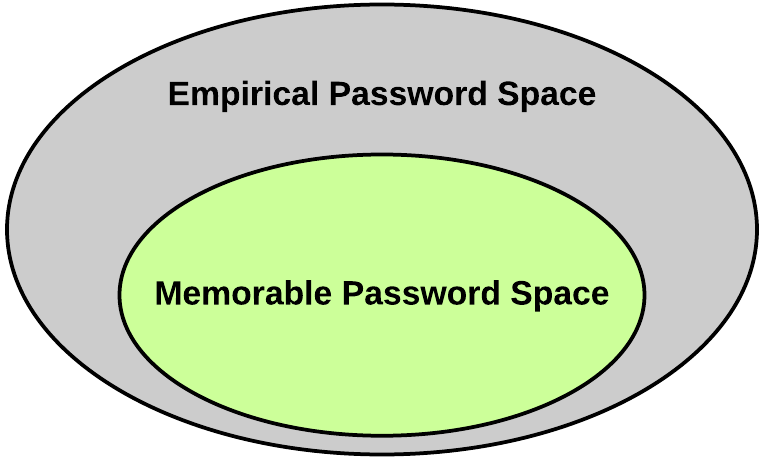
\includegraphics[scale=0.25]{pics/review/EmpiricalVsPractical.png}
      \caption{Empirical vs. Memorable Password Space}
      \label{fig:memorable}
    \end{figure}

  In a case study of 14.000 Unix passwords, a research group found a 25\% of the passwords were in a group of words forming a dictionary of $3\times10^{6}$ words \cite{UnixPasswords}. This dictionary shows that an attacker can have a relatively high success rate for an attack, despite the fact that there a roughly $2\times10^{14}$ 8-character passwords consisting of digits, and upper case and lower case letters. Due to the limitations of human memory, users often choose passwords that are easier to remember, causing a significant number of user-chosen password to fall into a small dictionary, e.g. practical password space \cite{Tao}. A well-designed dictionary is a tiny subset of the full password space, e.g. theoretical password space, which further can be prioritized according to the likelihood for a password to be chosen. It is, therefore, a commonly stated that the security of a password scheme is related closely to the size of its memorable/practical password space, rather than its theoretical password space. The high success rate of dictionary attack against textual passwords is believed to be strongly related to the recall capabilities of humans and how they choose their passwords, e.g. making meaningful and thus more easily remembered words are selected as passwords.

  One of the first large-scale studies on web password habits was conducted in 2007 by Microsoft research \cite{habits1}. They analyzed web password habits among 544960 Internet users over a period of 3 months. The data was collected from a Windows Live Toolbar, and they observed activities like login frequency. They also gathered information about the users age, the strength of the users passwords, as well as number of unique passwords and its use across different URLs. They observed that a typical user have an average of 7 distinct passwords and that an average of 5 of these passwords was re-used on different web pages. An estimate of the average number of account per user was estimated to be 25 accounts per user, but this would probably be higher since it seven years ago.

  Because of the shortcomings with a text-based authentication, graphical authentication are getting increased attention because it is an alternative to a text-based authentication trying to cope with the memorability and security issues of text-based password. Graphical passwords are using images and visual objects in the authentication instead of text and numeric values. When comparing text against visual objects, the human brain is more capable of remembering images than text. When the human brain is more suited for remembering images, the users might be able to remember more complicated passwords that are not easily guessed. To context where an authentication scheme is used have to be evaluated. Graphical passwords might not fit in all systems, but looks like a good alternative to mobile devices where the user interact with a touch sensitive screen. Typing a long text-based password on a small keyboard on a mobile device is not easy. When using, graphical passwords are easier to interact with on a small mobile screen.